\documentclass{standalone}

\usepackage{tikz}

\begin{document}

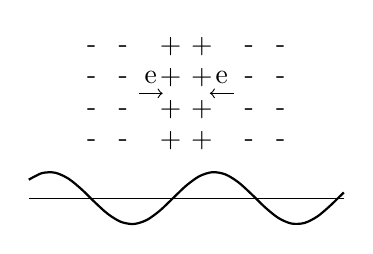
\begin{tikzpicture}

	\def\length{4}

	\draw (0, 0) -- (\length, 0);
	
	\def\amplitude{0.33}
	
	\draw[domain=0:\length, smooth, variable=\x, thick]
        plot ({\x}, {\amplitude*sin(3*deg(\x-pi/4+pi))});
        node[left] {E};
	
	\def\nx{2} % nombre de colonne de signe à mettre
	\def\ny{4} % nombre de lignes de signe à mettre
	
	\foreach \i in {1, ..., \nx} {
		\foreach	 \j in {1, ..., \ny} {
			\pgfmathsetmacro{\xposplus}{\length/4 + \i * \length/10 - 2*\length/10 + \length/10/\nx};
        	\pgfmathsetmacro{\xposminus}{\xposplus + \length/4};
        	\pgfmathsetmacro{\xposplusright}{\xposminus+\length/4};
        	\pgfmathsetmacro{\ypos}{\amplitude+\j*\length/10}
        
			\node at (\xposplus, \ypos) {-};
			\node at (\xposminus, \ypos) {+};
			\node at (\xposplusright, \ypos) {-};
		}
	}
	
	\draw[ <- ] (\length/2 - 1.25*\length/10 + \length/10/\nx, \amplitude+1.25*\ny*\length/20) -- (\length/4 + \nx * \length/10 - 2*\length/10 + 2*\length/10/\nx, \amplitude+1.25*\ny*\length/20) node[ midway, anchor=south ] {e};
	
	\draw[ <- ] (\length/2 + \nx*\length/10 - 2.5* \length/10/\nx, \amplitude+1.25*\ny*\length/20) -- (3*\length/4 + 0.5 * \length/10 - 2*\length/10 + \length/10/\nx, \amplitude+1.25*\ny*\length/20) node[ midway, anchor=south ] {e};

\end{tikzpicture}

\end{document}